\documentclass[english]{article}
\usepackage[T1]{fontenc}
\usepackage[utf8]{inputenc}
\usepackage{babel}
\usepackage{graphicx}
\usepackage{caption}
\usepackage{subcaption}
\usepackage{listings}

\newcommand{\design}{Nengo-RT}

\begin{document}

\lstset{basicstyle=\footnotesize}

\section{Introduction}

\subsection{Motivation}

\subsection{Potential Applications}

\subsection{State of the Art (Neuromorphic Hardware)}

\section{Methods}

\subsection{Description of NEF and population mode}

\subsubsection{Considerations related to hardware (multiplexing, clustering, using principal components)}

\subsection{High-level system description}

\design{} is a custom digital hardware design that implements the population-mode NEF in real-time (1~ms timestep).
% FIXME figure: block diagram
The encoder units perform the function of encoding (), % FIXME NEF equation
while the population units perform the decoding () % FIXME NEF equation
and write the decoded values to the decoded value buffers
to be used as inputs to other populations or as outputs from the network.
Each population of neurons is assigned to a population unit, which is able to simulate up to 1024 populations
having either one or two encoded inputs each. These inputs are calculated by the encoder units,
of which there are two for a one-dimensional population unit and four for a two-dimensional population unit.
Within each population unit, the decoder weights for each specific population are time-multiplexed
in order to run more populations on the same hardware, while the principal components are fixed and must be shared
between all populations on an individual population unit.
Each population unit writes to a fixed set of decoded value buffers, but a shared interconnect
allows the encoder units to perform random accesses to these buffers, which allows
inputs to a population to come from any combination of decoded values.
A number of decoded value buffers are reserved for external inputs to the network,
which can be sent from the controlling computer system over an Ethernet connection.
The output channels can also be programmed to send decoded values back to the computer over Ethernet.

\subsection{Hardware design details}

\subsubsection{Encoder Unit}

Each encoder unit communicates with the decoded value buffers over a shared interconnect, described below.
This is done in order to allow every encoder to read from every decoded value buffer.
However, because the decoded value buffers have a fixed number of access ports for reading data,
a maximum of two encoder units are allowed to access a single decoded value buffer simultaneously
without causing a bus collision.

Each encoder unit is attached to a circular buffer of size 8192 % FIXME check the size
containing a list of instructions for calculating one encoded value. 
This size was chosen as a compromise between memory utilization and encoder flexibility.
Each instruction corresponds to delaying for one or more clock cycles
(in order to coordinate concurrent access to the interconnect),
followed by reading one decoded value a certain address.
The decoded value data is made available to the encoder unit three clock cycles later
(due to interconnect delays), at which time it is multiplied by an encoder weight
and added to the accumulated encoded value, initially 0.
A certain bit in the instruction field acts as a flag to indicate that the encoded value is ready to be passed on to the population unit after this
instruction finishes executing. The encoder unit then waits for all other encoders to finish in order to synchronize
access to the shared interconnect, then resets the accumulator and begins encoding the next value.

The encoder units must each perform 1024 encoding operations per timestep.
To avoid duplication of logic, a single encoding controller connects to all encoder units and is responsible for
signalling them to start encoding when it detects that they have all finished encoding the previous value.
The encoding controller counts how many values have been encoded per timestep and
ensures that after 1024 such operations, the encoder units are not signalled to start again until
the beginning of the next timestep.

\subsubsection{Population Unit}

Encoded values are passed from the encoder units to the population units. Population units are either one-dimensional
(functions of one variable) or two-dimensional (functions of two variables).
Both types of population unit receive input from two encoder units in each input dimension;
for each dimension, the encoded values are passed through a separate first-order filter to simulate % FIXME ...post-synaptic time constant?
and then summed. The value resulting from this operation is
truncated to the most significant 10 bits and is then used as input to a set of lookup tables,
implemented as a bank of synchronous RAM elements. SRAMs are used
because the contents of these tables are not known until simulation-time and therefore the lookups cannot be implemented as hardware logic functions.
Each lookup table contains the 12-bit fixed-point values of points sampled from the principal components shared by all populations of neurons
simulated on that population unit. For one-dimensional population units, there are seven such lookup tables, and each one contains
1024 values sampled at equally-spaced points on the open interval $(-2, 2)$. For two-dimensional population units,
there are fifteen lookup tables, each containing 1024 values sampled at equally-spaced points on a square of width 4
centered at $(0, 0)$. The resulting sample space is a 32x32 grid.
To increase the accuracy of this representation, each two-dimensional population unit performs bilinear interpolation
using the least significant five bits of each input variable to determine the distance between sample points. 
The extra resources used to perform this operation are modest
and significantly reduce the amount of memory used for two-dimensional populations while maintaining a good degree of accuracy of representation.

To simulate the noise resulting from a neural representation, a pseudorandom Gaussian noise generator is implemented in each population unit.
The output from the noise generator is passed through a programmable second-order filter to approximate the power spectrum of the noise
that would be present if individual neurons were being implemented. % FIXME fact check and possibly get a citation

The interpolated values from the principal component lookup tables and the filtered noise sample are multiplied by a vector of decoders,
and these results are summed to produce a decoded value. Each population unit can store up to four independent sets of decoders per population being simulated,
which allows each population to produce a maximum of four decoded values as some function of its inputs
(and the resulting values of its principal components).

\subsubsection{Decoded Value Buffers and Interconnect}

Decoded values calculated from population units are stored in decoded value buffers, which are fairly large memory banks that can each
store 2048 decoded values. The buffers themselves expose a read-only interface, accessed by the encoders to read decoded values from the
previous timestep, and a write-only interface, accessed by the population units when new decoded values are calculated.
Internally, each interface is connected to a separate dual-port RAM; the connections are swapped between RAMs
at the end of each timestep in order to implement double-buffering, so that it is not possible for encoders to read a
partially-updated set of decoded values, where some are from the previous timestep and some are freshly written during the current timestep.
% FIXME DV double buffer diagram in here somewhere
Because each population unit produces 4096 decoded values (1024 DVs from each of four decoder vectors),
this means that a population unit must be attached to the write-only interfaces of two separate decoded value buffers.

The encoders must share access to the read-only interface of the decoded value buffers. To accomplish this,
the encoders are connected to the decoded value buffers over a shared interconnect. Access to the decoded value buffers
is managed by arbiters that inspect the decoded values being read from by encoders and redirect the read operations to the
corresponding buffers. A maximum of two encoders may be accessing a single buffer at any one time.
Therefore, it is up to the compiler to generate a sequence of read instructions for the encoders that ensures that this
constraint is respected. The delay field in the encoder instruction word can be used for this purpose to make an encoder
wait until another is finished with its access before attempting to read from the same buffer.

\subsubsection{Input, Output, and Control}

A number of decoded value buffers are set aside for use as inputs to the simulation. These are indistinguishable from other decoded value buffers
from the perspective of the encoders and interconnect, but instead of being written to by population units,
they are connected to one or more input channels which are responsible for receiving data from an external source
and writing it to the buffers.

To provide output to an external source, such as a simulation GUI running on a computer, one or more output channels
can be implemented whose function is to read from the decoded value buffers and output the desired decoded values to be transmitted
to an external device. Output channels do not have access to the interconnect until all encoders have finished all
encoding operations for this timestep. At that point, the encoders are detached from the interconnect by a separate controller and the output
channels are attached in their place. This allows the output channels to share interconnect logic with the encoders;
it also increases efficiency both by reducing contention on the shared interconnect (as the encoders and output channels
do not access it at the same time) and by allowing output to happen at the same time as decoding
(the double-buffering of decoded values means that output channels always see a consistent set of values,
so these operations can be performed in parallel).

Both the input and output channels are transport-agnostic and can be attached to application-specific custom hardware that allows for
I/O to be performed over the desired interface, such as Ethernet. The implemented design performs I/O over Gigabit Ethernet using a custom Ethernet frame format for efficiency.

The top-level module exposes a programming interface that allows for any of the runtime configurable components
(decoded value buffers, encoders, population unit filters, principal component lookup tables,
population unit noise generators, decoder vectors, and I/O channels) to be initialized and programmed
over an external interface such as Ethernet. This allows a single implementation of the design
to be used to simulate a large number of different neural networks without requiring modifications to the physical hardware.
The programming interface also allows an external controller to reset the hardware and to start, pause, or single-step a simulation
without requiring physical access to the hardware.

\subsection{Constraints on models}

There is an artificial limitation on the complexity of the encoding operation due to the length of the instruction buffer that is used.
Because each encoder must produce 1024 encoded values per timestep, using an instruction memory of size 8192 for each encoder means that a maximum of eight decoded values
can be used as input to each encoder per population.
It is theoretically possible to simulate populations that require more than eight decoded values to be read by a single encoder,
but the extra instructions used for this mean that other populations sharing that encoder will have to use fewer.
It is expected that the compiler will be able to detect this scenario and reorganize populations appropriately so as to avoid overfilling the instruction buffers.

% FIXME citation about why 2D is ``good enough''
As only one-dimensional and two-dimensional population units have been implemented, networks that require populations to compute functions
of three or more independent variables cannot be simulated with this design.

The choice of using a maximum of four sets of decoder vectors per population is arbitrary; it seems to be a good balance between
population connectivity and memory usage. However, populations that have more than four outgoing connections must be treated specially.
Assuming none of the outgoing connections can be combined together (for example, if the function they decode only differs by a constant),
in order to implement such a population on the simulator, it is necessary to duplicate it and simulate it twice,
once with the first four decoder vectors and again with the remaining ones. The consequence of this is that a population with more than
four outgoing connections will be represented as two or more populations in simulation, thereby reducing the actual number of
distinct populations that can be simulated.

\subsection{Implementation details}

\begin{itemize}
\item VC707 board
\item resources available -- BRAM, DSP
\item implemented design -- number of population units, DV buffers
\item FPGA resources utilized; maximum theoretical design size
\item clock speed and implications of this
\item Ethernet communication for control and I/O -- maximum channel capacity in terms of DVs
\end{itemize}

\subsection{Nengo backend}

\begin{itemize}
\item quick description of Nengo
\item Nengo ensembles are hardware populations
\item Nengo connections are hardware encoders and decoders
\item Nengo nodes and probes are hardware I/O endpoints
\item compiler functions: calculate principal components, map populations to PCs, calculate decoders and encoders,
calculate encoder schedule, create programming file
\item Nengo will then program the board and communicate with it during simulation
\end{itemize}

\section{Results}

To verify the correct operation of the hardware as well as the software backend to Nengo, a simple network consisting of a single neural integrator was compiled and simulated on the hardware.
Figure~\ref{lst:integrator1d} shows the code listing and the resulting network that it describes.
\begin{figure}
\centering

\begin{subfigure}[b]{\textwidth}
\centering
\lstset{language=Python}
\begin{lstlisting}[frame=single]
import nengo
import nengo.helpers
model = nengo.Model(label='Integrator')
input = nengo.Node(nengo.helpers.piecewise({0:0.5}), label='Input')
tau = 0.1
A = nengo.Ensemble(nengo.LIF(100, tau_rc=0.02, tau_ref=0.002,
                   dimensions=1, label='Integrator'))
nengo.Connection(A, A, transform=[[1]], filter=tau)
nengo.Connection(input, A, transform=[[tau]], filter=tau)
p1 = nengo.Probe(input, 'output')
p2 = nengo.Probe(A, 'decoded_output', filter=0.01)
\end{lstlisting}
\caption{Source code}
\label{lst:integrator1d:code}
\end{subfigure}

\begin{subfigure}[b]{0.3\textwidth}
\centering
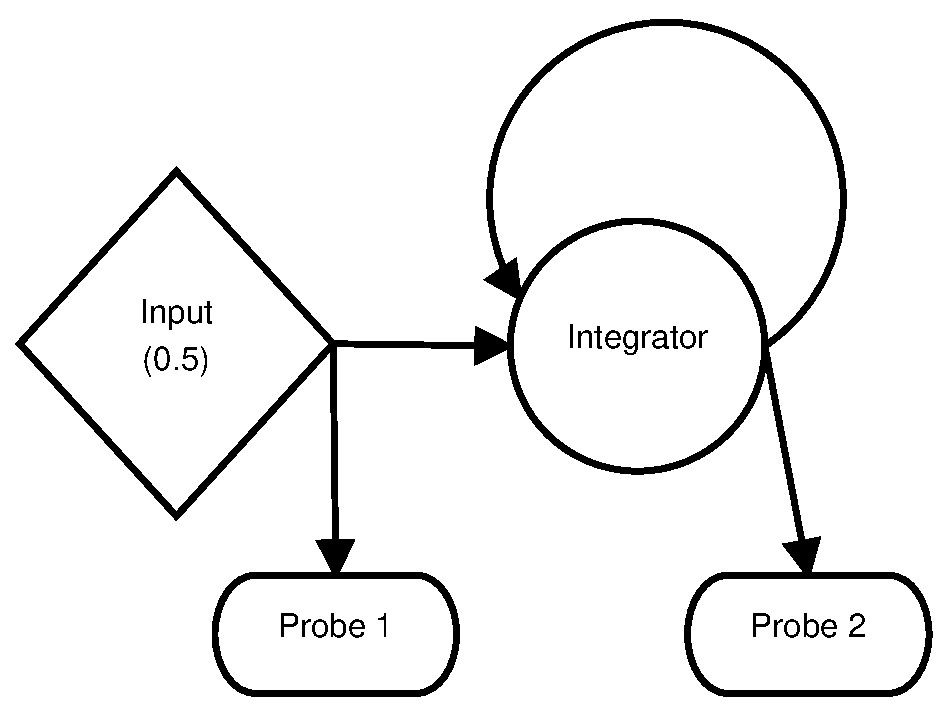
\includegraphics[width=3.0in]{integrator-1d-schematic.eps}
\caption{Schematic}
\label{lst:integrator1d:schematic}
\end{subfigure}

\caption[A 1D neural integrator in Nengo.]
{Source code (\ref{lst:integrator1d:code}) and schematic (\ref{lst:integrator1d:schematic}) of a 1D neural integrator in Nengo.}
\label{lst:integrator1d}
\end{figure}

% FIXME explanation of the code?
The network was compiled with the \design{} backend to produce a programming file that could be used to configure the simulator hardware.
Simulation output from the FPGA was captured with an Ethernet traffic sniffer and plotted in Figure~\ref{fig:integrator1d}.

\begin{figure}
\centering

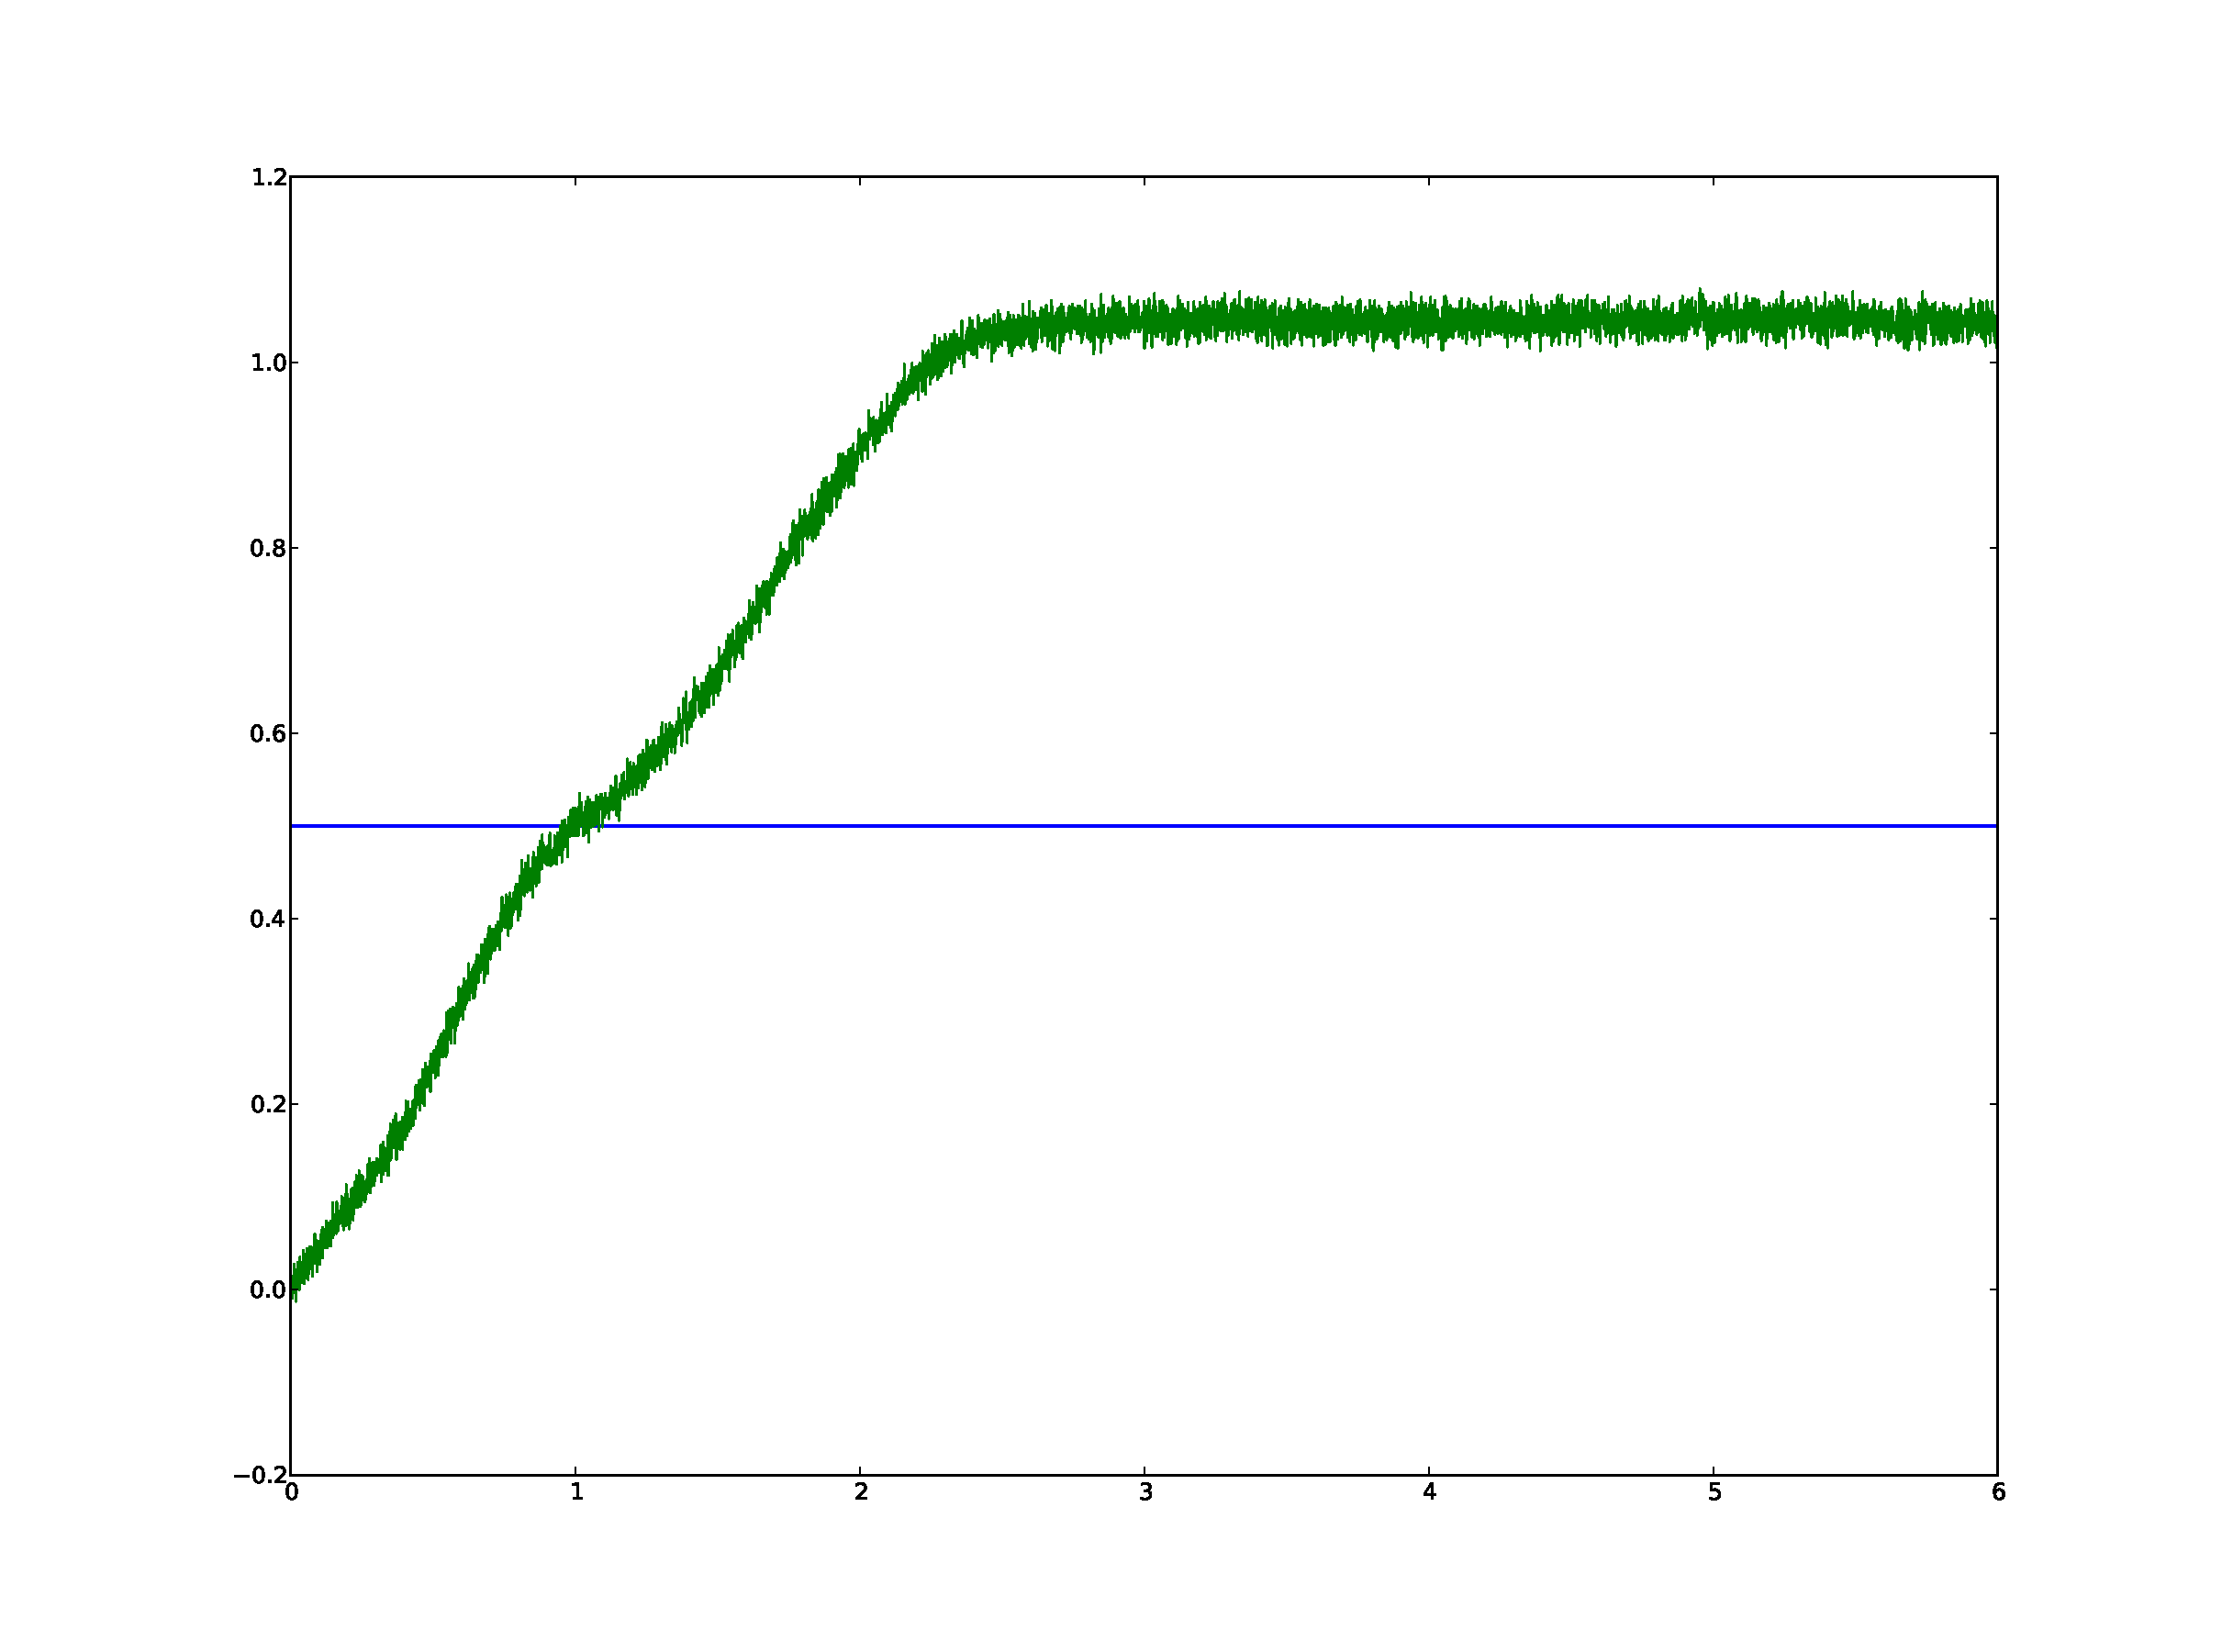
\includegraphics[width=6in]{integrator-1d.eps}

\caption[Simulation of a 1D neural integrator.]
{Hardware output from simulation of a one-dimensional population representing a neural integrator.}

\label{fig:integrator1d}
\end{figure}

% FIXME discussion of result?

\subsection{elaborate simulations}

\subsection{power, \% timestep used for each simulation, \% of board resources for each simulation}

\section{Discussion}

\subsection{How well it worked}

\subsection{Limitations}

\subsection{Future work \& extensions}

\begin{itemize}
\item board-to-board communication for larger networks

The flexibility of input and output channels lends to their use in connecting multiple devices together for use as part of a larger simulation engine.
This would allow networks to be simulated that consume more resources than are available on a single device, which may in turn allow
for ``grids'' of inexpensive hardware devices to be used to simulate a very large model.
\item increase design size by using off-chip memory (DDR3)
\item better network stack to allow control and I/O over common protocols e.g. UDP

The current control and I/O interface communicates over Ethernet, but since bare frames are being used with no higher-level protocols on top of them,
it is somewhat cumbersome to set up a computer or other device to send and receive data to the hardware.
This approach is suitable for testing and prototyping, but it makes certain assumptions about the setup of the network and the host computer that
may not be reasonable for general use, such as requiring raw socket privileges on the host operating system (which typically require administrator access).
A more user-friendly approach would be to implement an Ethernet stack that supports a protocol such as UDP, which can be readily used by many different
kinds of host software in order to interact with a simulation.
\end{itemize}

\end{document}
